\subsection{Co-Simulations and SIL / HIL}

Co-simulations are used to model and analyze complex systems with multiple
interacting components, each of which may have different properties and
behaviors. They involve combining simulation models from different domains, such
as control, power, and thermal management, to create a unified model that
accurately represents the behavior of the overall system.

One of the main advantages of co-simulations over regular simulations is their
ability to capture the interactions between different components of the system.
Regular simulations often make simplifying assumptions that can lead to
inaccurate results. Co-simulations, on the other hand, can account for the
interactions between components and provide a more accurate representation of
the system's behavior. This makes co-simulations particularly useful for
designing and optimizing complex systems like datacenters. The virtual
environment can save time and resources, reduce the risk of failure, and lead to
more efficient and sustainable datacenters \cite{vogt2018}.

Co-simulations can be further enhanced by incorporating the SIL and HIL
methodology. This approach involves integrating real-world components, such as
software and hardware, into the simulation environment to better reflect the
actual system behavior. The integration of real components allows for a more
accurate representation of the system's behavior and can also identify potential
issues that may arise in real-world scenarios \cite{kelemenova2013}.

\subsection{Mosaik}

Mosaik is an open-source co-simulation tool that allows for the integration of
different simulation models from various domains into a unified simulation
environment \cite{steinbrink2019}. Mosaik’s four main components enable
communication between simulators and Mosaik, the creation of simulation
scenarios, the management of simulator processes, and the coordinated simulation
of a scenario.\footnote{The information about the main components is adapted
from the official documentation \cite{mosaik_docs}.}

\begin{description}

    \item[Mosaik Sim API.] The Mosaik Sim API provides a standardized
        communication protocol for simulators and Mosaik to exchange
        information. It utilizes plain network sockets and JSON encoded messages
        to facilitate communication between simulators and Mosaik. Although the
        API provides a low-level communication protocol, it is complemented by a
        high-level API for some programming languages. The high-level API
        abstracts the networking-related aspects of the communication protocol,
        allowing users to focus on the core logic of their simulation models. To
        use the high-level API, users only need to write a subclass and
        implement a few required methods.

    \item[Scenario API.] This empowers users to create simulation scenarios
        entirely in Python. This API enables users to launch simulators, create
        model instances, and generate entity sets that can be connected to
        establish data flows between different simulators. With the Scenario
        API, users can easily connect individual entities or entire sets of
        entities to achieve their simulation goals.

    \item[SimManager.] The Simulator Manager, or SimManager, handles simulator
        processes and their communication with Mosaik. The SimManager can start
        new simulator processes, connect to already running process instances,
        and import a simulator module and execute it in-process if it is written
        in Python 3. In-process execution reduces memory requirements and avoids
        the overhead of serializing and sending messages over the network.
        External processes, however, can be executed in parallel, which is not
        possible with in-process simulators.

    \item[Mosaik's Scheduler.] Mosaik's Scheduler uses the event-discrete
        simulation library SimPy for the coordinated simulation of a scenario.
        Mosaik supports time-discrete and event-discrete simulations, as well as
        a combination of both paradigms. It can handle simulators with different
        step sizes, and a simulator may vary its step size during the
        simulation. Mosaik tracks the dependencies between simulators and only
        lets them perform a simulation step if necessary. It is also able to let
        multiple simulators perform their simulation step in parallel if they do
        not depend on each other's data.

\end{description}

\subsection[Ecovisor]{
    Ecovisor \footnote{The information presented in this section is a summary of
    Section 3 and 3.1 from Souza et al.'s work \cite{souza2023}, with some
    modifications made for clarity and conciseness.}
}

Figure \ref{fig:ecovisor_design} shows an overview of the ecovisor's design
which manages resources and energy using containers or virtual machines as the
basic unit. An instance-level API is chosen to align with existing cloud APIs
and to support higher-level cluster or cloud-level APIs. The ecovisor extends an
existing orchestration platform that provides basic container or VM management
and monitoring functions. Container Orchestration Platforms (COPs) are used to
manage resources and applications. COPs provide virtual clusters composed of
multiple containers with specified resource allocations that can grow or shrink
over time. COPs include a scheduling policy that determines resource allocation
under constraints, and COPs are resilient to resource revocations. This
resiliency is useful for designing carbon-efficient applications as low-carbon
energy may cause power shortages that also manifest as resource revocations.

The virtual energy system includes a virtual grid connection, a virtual battery,
and a virtual solar array. The system provides getters and setters methods for
monitoring and controlling the virtual power supply and demand, including
per-container power caps, battery charging, and discharging rates, as shown in
Table \ref{table:ecovisor_api}. The system uses virtual solar power first to
meet demand and charges the virtual battery with any excess solar power. When
there is not enough solar power, the virtual energy system uses grid power to
make up the difference, while accounting for carbon emissions and power usage
over discrete time intervals. The ecovisor system provides a uniform centralized
interface for accessing energy-related information and historical data.

\begin{figure}
    \centering
    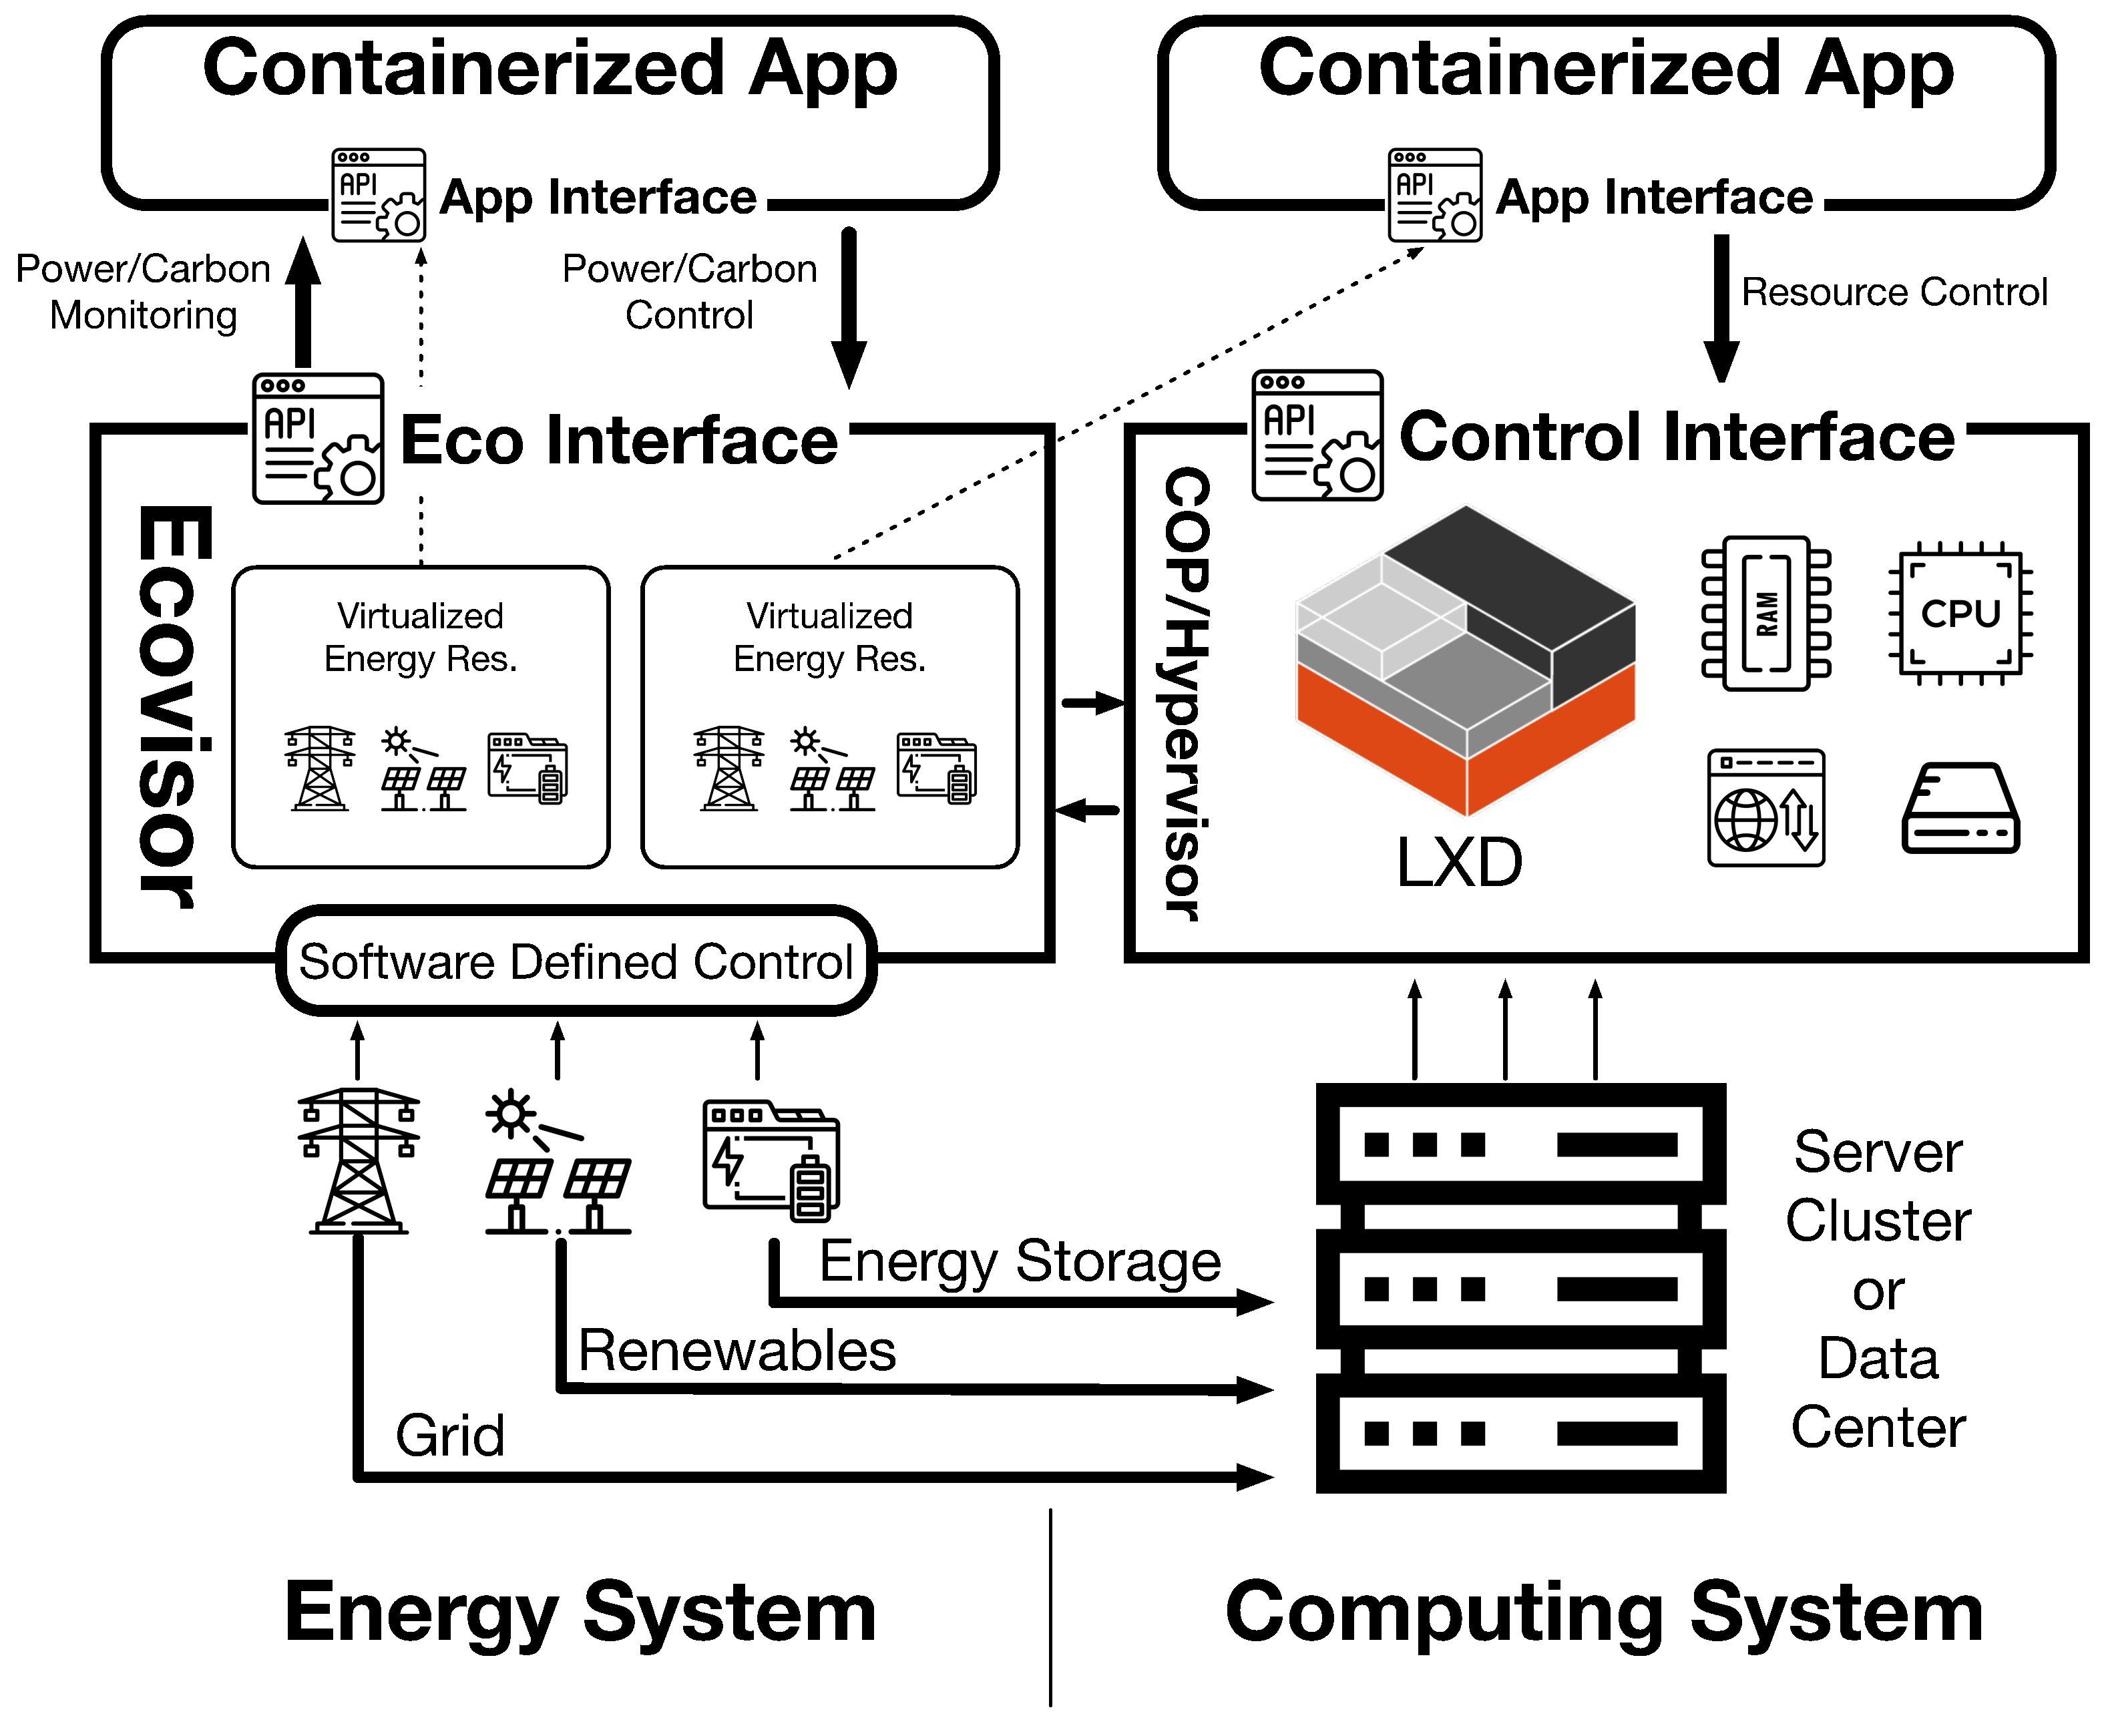
\includegraphics[width=\linewidth]{figures/ecovisor_design}
    \caption{Ecovisor Design (Souza et al.) \cite{souza2023}}
    \label{fig:ecovisor_design}
\end{figure}

\begin{table*}
    \centering
    \caption{Ecovisor's API (Souza et al.) \cite{souza2023}}
    \label{table:ecovisor_api}
    \begin{tabular}{||l|c|c|c|c||}
        \hline
        \textbf{Function Name} & \textbf{Type} & \textbf{Input} & \textbf{Return
        Value} & \textbf{Description} \\
        \hline\hline
        \texttt{set\_container\_powercap()} & Setter & ContainerID, kW & N/A & Set
        a container's power cap \\
        \hline
        \texttt{set\_battery\_charge\_rate()} & Setter & kW & N/A & Set battery charge rate until full \\
        \hline
        \texttt{set\_battery\_max\_discharge()} & Setter & kW & N/A & Set max battery discharge rate \\
        \hline\hline\hline
        \texttt{get\_solar\_power()} & Getter & N/A & kW & Get virtual solar power output \\
        \hline
        \texttt{get\_grid\_power()} & Getter & N/A & kW & Get virtual grid power usage \\
        \hline
        \texttt{get\_grid\_carbon()} & Getter & N/A &
        g\,$\cdot$\,CO\textsubscript{2}/kW & Get virtual grid power usage \\
        \hline
        \texttt{get\_battery\_discharge\_rate()} & Getter & N/A & kW & Get current rate of battery discharge \\
        \hline
        \texttt{get\_battery\_charge\_level()} & Getter & N/A & kWh & Get energy
        stored in virtual battery \\
        \hline
        \texttt{get\_container\_powercap()} & Getter & ContainerID & kW & Get a
        container's power cap \\
        \hline
        \texttt{get\_container\_power()} & Getter & ContainerID & kW & Get a
        container's power usage \\
        \hline\hline\hline
        \texttt{tick()} & Notification & N/A & N/A & Invoked by ecovisor every
        $\Delta t$ \\
        \hline
    \end{tabular}
\end{table*}
